\section{Simulation Experiments and Results}
\label{sec:simulation_experiments}

We now present four example tasks to demonstrate our algorithm, two with cloth, and two with rope. These tasks are designed to show that our framework is able to handle non-trivial tasks which cannot be performed using either our controller or planner alone. In Section~\ref{sec:live_robot} we demonstrate that our method can also be applied to a physical robot.

For these simulation tasks $\robotCspace = \gripperCspace$ -- i.e. there are two free flying grippers. In the first and second tasks, two grippers manipulate the cloth so that it covers a table. In the first task the cloth is obstructed by a pillar while in the second task the grippers must pass through a narrow passage before the table can be covered. The third and fourth scenarios require the robot to navigate a rope through a three-dimensional maze before aligning the rope with a line traced on the floor (see Figure~\ref{fig:example_tasks}). A video showing the experiments can be found at \ijrrurl.

All experiments were conducted in the open-source Bullet simulator \cite{Coumans2010}, with additional wrapper code developed at UC Berkeley~\cite{ucberkley_bullet}. The cloth is modeled as a triangle mesh using 1500 vertices with a total size of $0.3\text{m} \times 0.5\text{m}$. The rope is modeled as a series of small capsules linked together by springs. In the first rope experiment we use 39 capsules for a 0.78m long rope, and 47 capsules for a 0.94m rope in the last experiment. We emphasize that our method does not have access to the model of the deformable object or the simulation parameters. The simulator is used as a ``black box'' for testing. We set the maximum stretching factor $\stretchmax$ to 1.17 for the cloth and 1.15 for the rope. All tests are performed using an i7-8700K 3.7 GHz CPU with 32 GB of RAM. We use the same deadlock prediction and planner parameters for all tasks, shown in Tables~\ref{tab:deadlock_param_table} and~\ref{tab:rrt_param_table}. For the purpose of the planner we treat the grippers as spheres, reducing the planning space from $\gripperCspace \times \bandspace$ to $\reals^6 \times \bandspace$.

\begin{table}[h]
\centering
\caption{Deadlock prediction parameters}
\label{tab:deadlock_param_table}
\begin{tabular}{lcc}
\noalign{\smallskip}\hline\noalign{\smallskip}
Prediction Horizon                  & $\predictionhorizon$          &    10 \\
Band Annealing Factor               & $\bandlengthannealing$        &   0.3 \\
History Window                      & $\historywindow$              &   100 \\
Error Improvement Threshold         & $\errorprogressthreshold$     &     1 \\
Configuration Distance Threshold    & $\motionprogressthreshold$    &  0.03 \\
\noalign{\smallskip}\hline
\end{tabular}
\end{table}


\begin{table}[h]
\centering
\caption{Distance and planner parameters}
\label{tab:rrt_param_table}
\begin{tabular}{lcc}
\noalign{\smallskip}\hline\noalign{\smallskip}
Goal Bias                           & $\goalbias$                   &     0.1 \\
Workspace Goal Radius               & $\eegoalradius$               &     0.02 \\
Best Nearest Radius                 & $\bestneardist$               &     0.001 \\
Band Distance Scaling Factor        & $\banddistscale$              & $10^{-6}$ \\
Maximum Band Points                 & $\nbandpointsmax$             & 500 \\
\noalign{\smallskip}\hline
\end{tabular}
\end{table}

To smooth the path returned by the planner, at each iteration we randomly select either a single gripper or both grippers and two configurations in the path. To smooth between the configurations we use the same forward-propagation method for the VEB as used in the planning process. If we have selected only one gripper for smoothing, we do not change the configuration of the second gripper during that smoothing iteration. We also forward-propagate the VEB to the end of the path to ensure that the band at the end of the smoothed path is dissimilar from the blacklist. We perform 500 smoothing iterations for experiments 1, 2, and 4; and 1500 for experiment 3 due to the larger environment.


\subsection{Single Pillar}
\label{sec:single_pillar}

In the first example task, the objective is to spread the cloth across a table that is on the far side  of a pillar (see Figure~\ref{fig:cloth_single_pole}). We uniformly discretize the surface of the table to create the target points $\target$, with each discretized point creating a navigation function that pulls the closest point on the deformable object towards the target. These target points are set slightly above the surface to allow for collision margins within the simulator. A single point on the cloth can have multiple ``pulls'' or none. Task error $\ErrorFn$ is defined as the sum of the Dijkstra's distances from each target point to the closest point on the cloth. If a target point in $\target$ is within a small-enough threshold of their nearest neighbors in $\deformconfig$, then these points are considered ``covered'' and do not influence task error or any other calculation. Our results show that even though the global planner is only planning using the gripper positions and a VEB between them, it is able to find the correct neighbourhood for the local controller to complete the task. On average we are able to find and smooth a path in 3.0 seconds (Table~\ref{tab:planning_statistics}, Table~\ref{tab:smoothing_statistics}), with the majority of the planning time spent on forward propagation of the VEB as part of the validity check for a potential movement of the grippers. In all 100 trials the global planner is only invoked once, with the local controller completing the task after the plan finishes.

\begin{figure}[h]
    \centering
    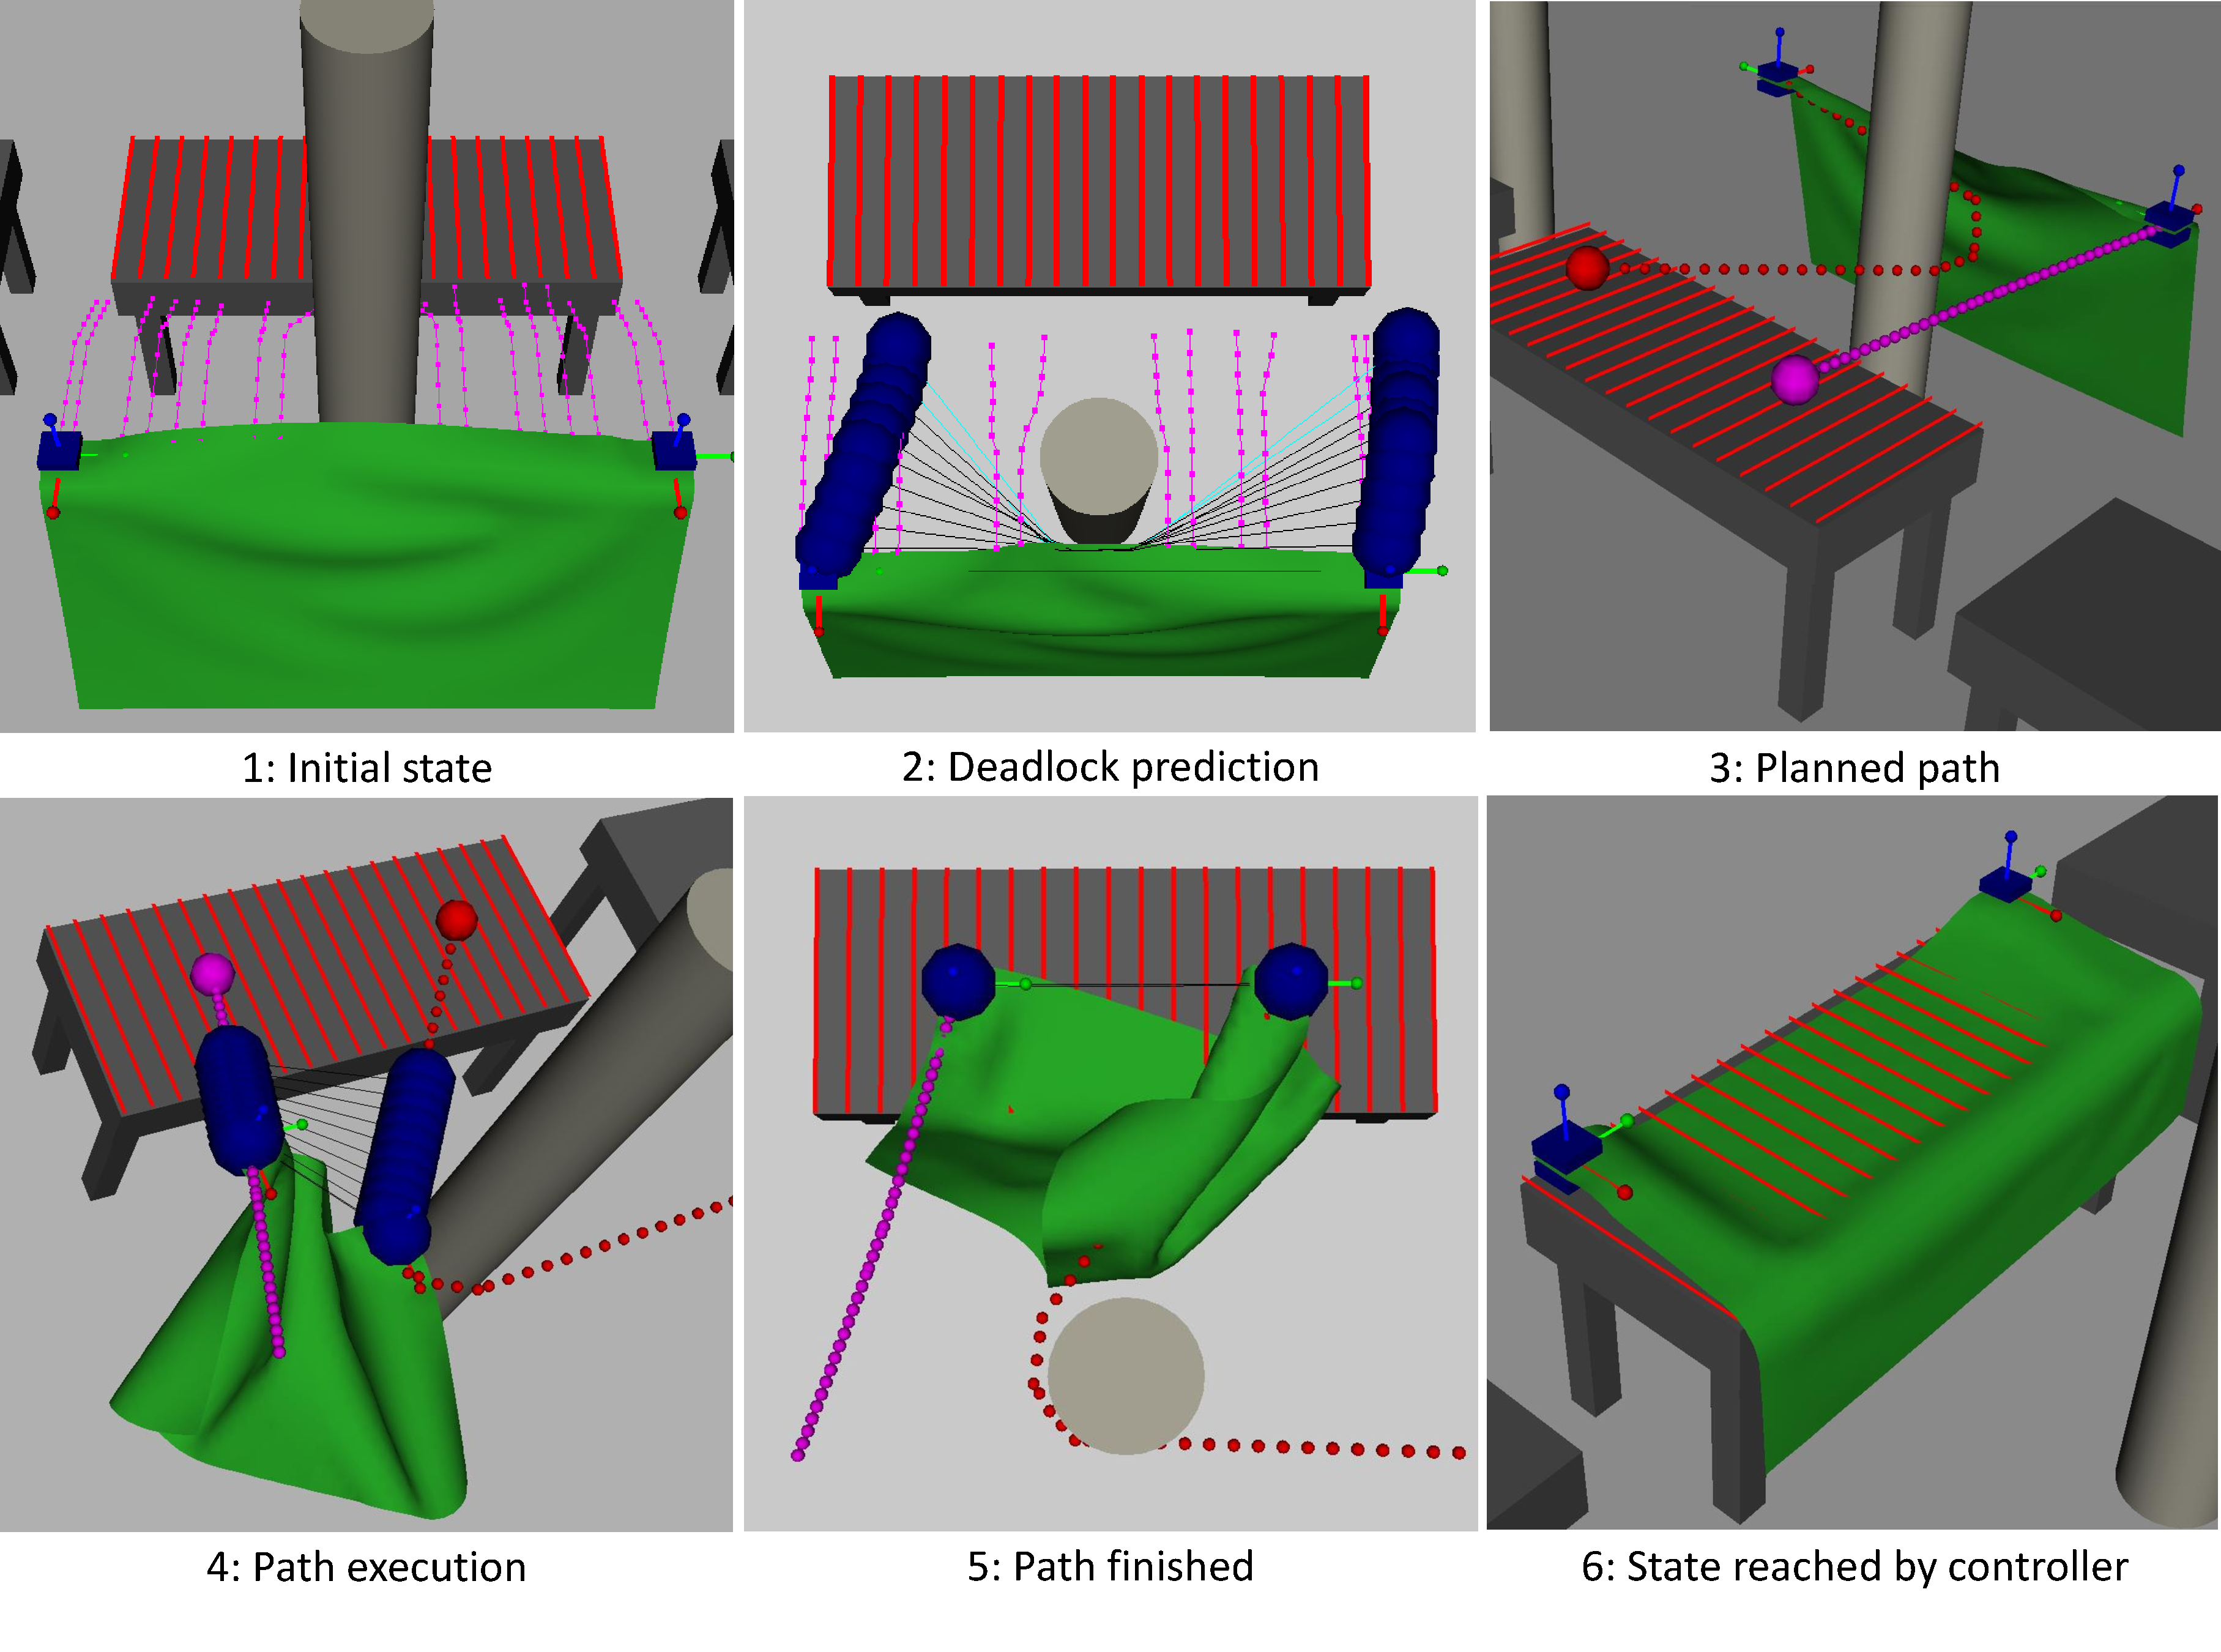
\includegraphics[width=\textwidth]{CombinedImages_ClothSinglePole}
    \vspace{-0.2in}
    \caption{Sequence of snapshots showing the execution of the first experiment. The cloth is shown in green, the grippers are shown in blue, and the target points are shown as red lines. (1) The approximate integration of the navigation functions from error reduction over $\predictionhorizon$ timesteps, shown in magenta, pull the cloth to opposite sides of the pillar. (2) A sequence of VEBs between the grippers is shown in black and teal, indicating the predicted gripper configuration over the prediction horizon as the local controller follows the navigation functions. The elastic band changes to teal as the predicted motion of the grippers moves the cloth into an infeasible configuration. (3 - 5) The resulting plan by the RRT, shown in magenta and red, moves the system into a new neighbourhood. (6) Final system state when the task is finished by the local controller.}
    \label{fig:cloth_single_pole}
\end{figure}

\FloatBarrier

\subsection{Double Slit}
\label{sec:double_slit}
The second experiment uses the same setup as the first, with the only change being that the single pillar obstacle is replaced by a wide wall with two narrow slits (Figure~\ref{fig:cloth_double_slit}). This adds a narrow passage problem and also demonstrates the utility of the progress detection filter. In this example the local controller is trying to move the deformable object straight forward, but with the wall in the way it is unable to make progress; the local controller cannot explicitly go around obstacles. This experiment shows comparable planning time, but it takes longer to smooth the resulting path (as expected given that the VEB forward propagation takes longer near obstacles). The local controller is again able to complete the task after invoking the planer a single time on all 100 trials.

\begin{figure}[h]
    \centering
    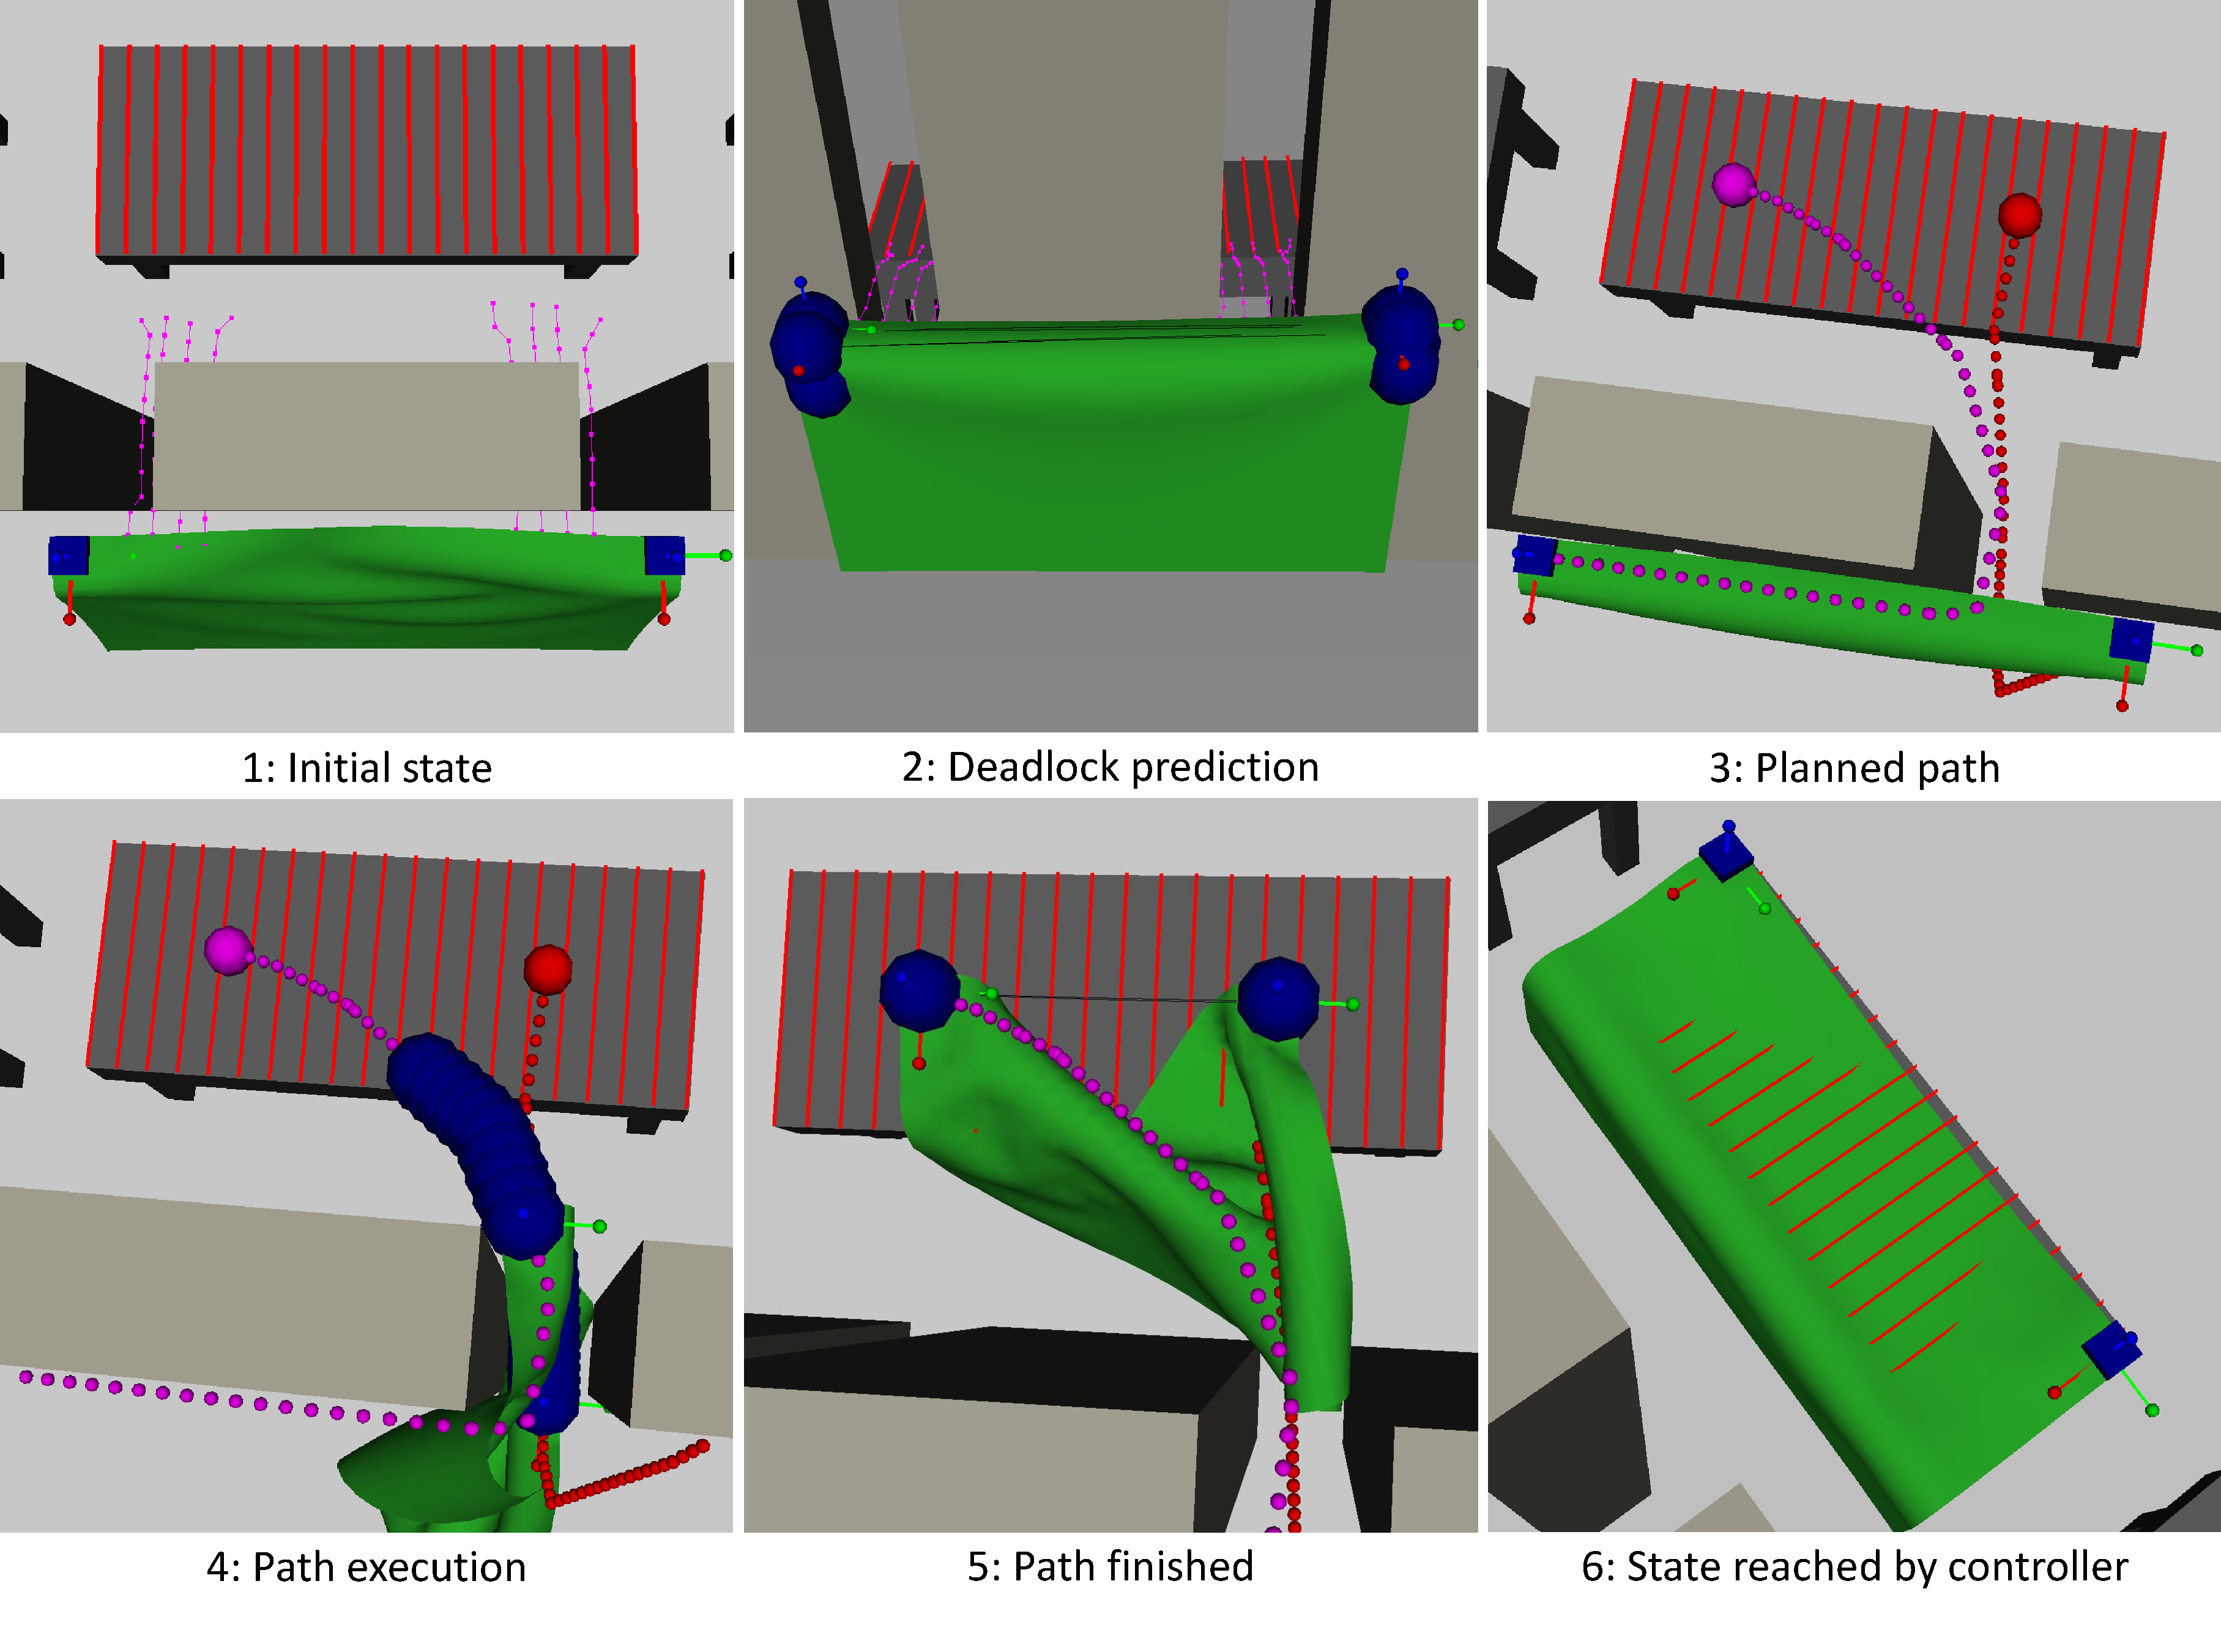
\includegraphics[width=\textwidth]{CombinedImages_ClothDoubleSlit}
    \vspace{-0.2in}
    \caption{Sequence of snapshots showing the execution of the second experiment. We use the same colors as the previous experiment (Figure~\ref{fig:cloth_single_pole}), but in this example instead of detecting future overstretch in panel (2), we detect that the system is stuck in a bad local minimum and unable to make progress.}
    \label{fig:cloth_double_slit}
\end{figure}

\FloatBarrier

\subsection{Moving a Rope Through a Maze}
\label{sec:rope_maze}
In the third task, the robot must navigate a rope through a three-dimensional maze before aligning the rope with a line traced on the floor (Figure~\ref{fig:rope_maze}). This scenario is meant to represent tasks such as moving a heavy cable through a construction zone without crane access. In this task, the correspondences between the target points $\target$ and the deformable object points $\deformconfig$ are fixed in advance, thus the CalculateCorrespondences() function does not have to do any work, as shown in Table~\ref{tab:control_statistics}. Task error $\ErrorFn$ is defined in the same way as in the first two experiments. Again the planner is invoked a single time per trial, but planning and smoothing times are longer than the previous tasks. This is a function of the size of the environment rather than any particular difference in the difficulty of performing the planning or smoothing. The planner finds a feasible path in 4.2s on average, suggesting that our method can maintain fast planning times, even in larger environments with many more obstacles.

\begin{figure}[h]
    \centering
    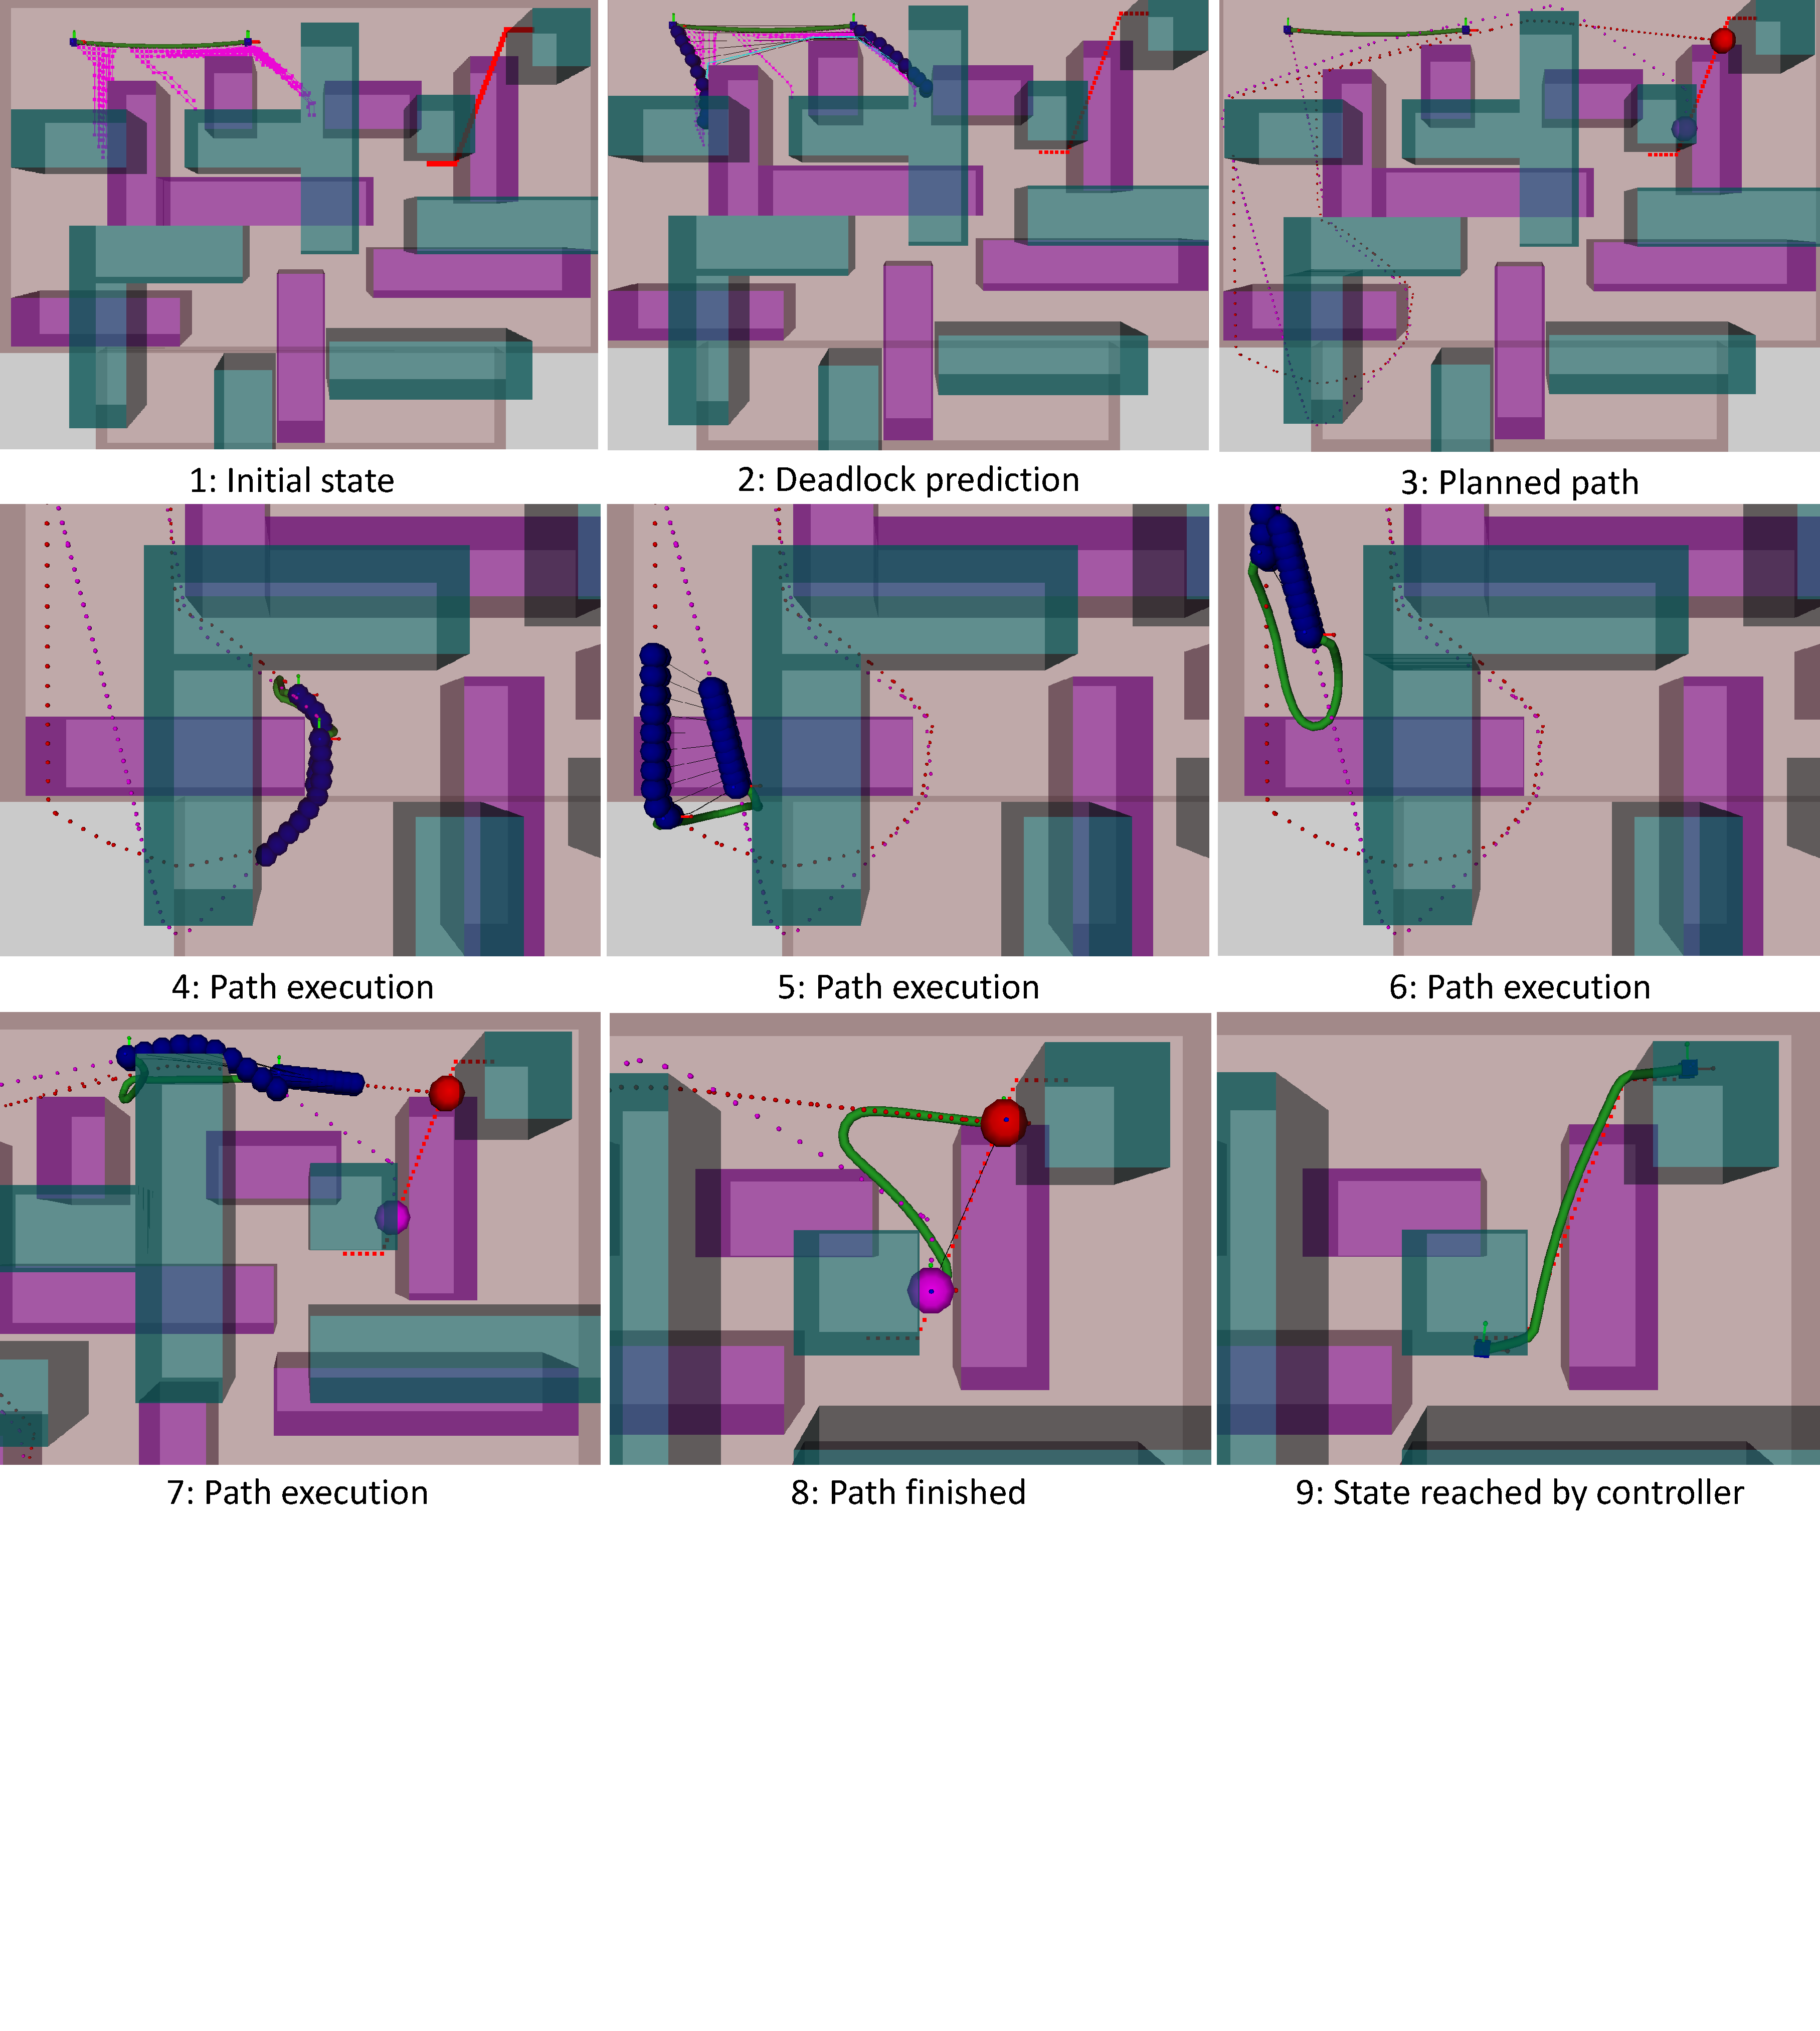
\includegraphics[width=\textwidth]{CombinedImages_RopeMaze}
    \vspace{-2in}
    \caption{Sequence of snapshots showing the execution of the third experiment. The rope is shown in green starting in the top left corner, the grippers are shown in blue, and the target points are shown in red in the top right corner. The maze consists of top and bottom layers (green and purple, respectively). The rope starts in the bottom layer and must move to the target on the top layer through an opening (bottom left or bottom right).}
    \label{fig:rope_maze}
\end{figure}

\FloatBarrier

\subsection{Repeated Planning}
\label{sec:repeated_rope_maze}

The fourth task is a variant of the third, with the start configuration of the rope moved near the goal region on the top layer of the maze and a longer rope. This task has the most potential for a planned path to move the deformable object into a configuration from which the local controller cannot finish the task by wrapping the rope around an obstacle near the goal. For this experiment we reduce the size of the planning arena to only the goal area, and the immediate surroundings on the top layer (Figure~\ref{fig:repeated_planning}). From this starting position, the planner is more likely to find the incorrect neighborhood for the local controller, which corresponds to placing the rope into the wrong homotopy class, on the first attempt. We emphasize that the correct homotopy class is unknown, as we assume no information is given about the connectivity of the target points. Thus our method must discover the correct homotopy class by trail-and-error, invoking the planner when the deadlock prediction determines the controller will be stuck.

In 71 of the 100 trials, the planner was invoked twice, in 13 other trials it was invoked three times, and in 2 trials it was invoked four times. These additional planning and smoothing stages took on average an additional 6.6 seconds, but the task was completed successfully in all 100 trials. This experiment suggests that our framework is able to effectively explore different band neighborhoods until the correct one is found, enabling the local controller to finish the task, even when the initial configuration is adversarial.

\begin{figure}[h]
    \centering
    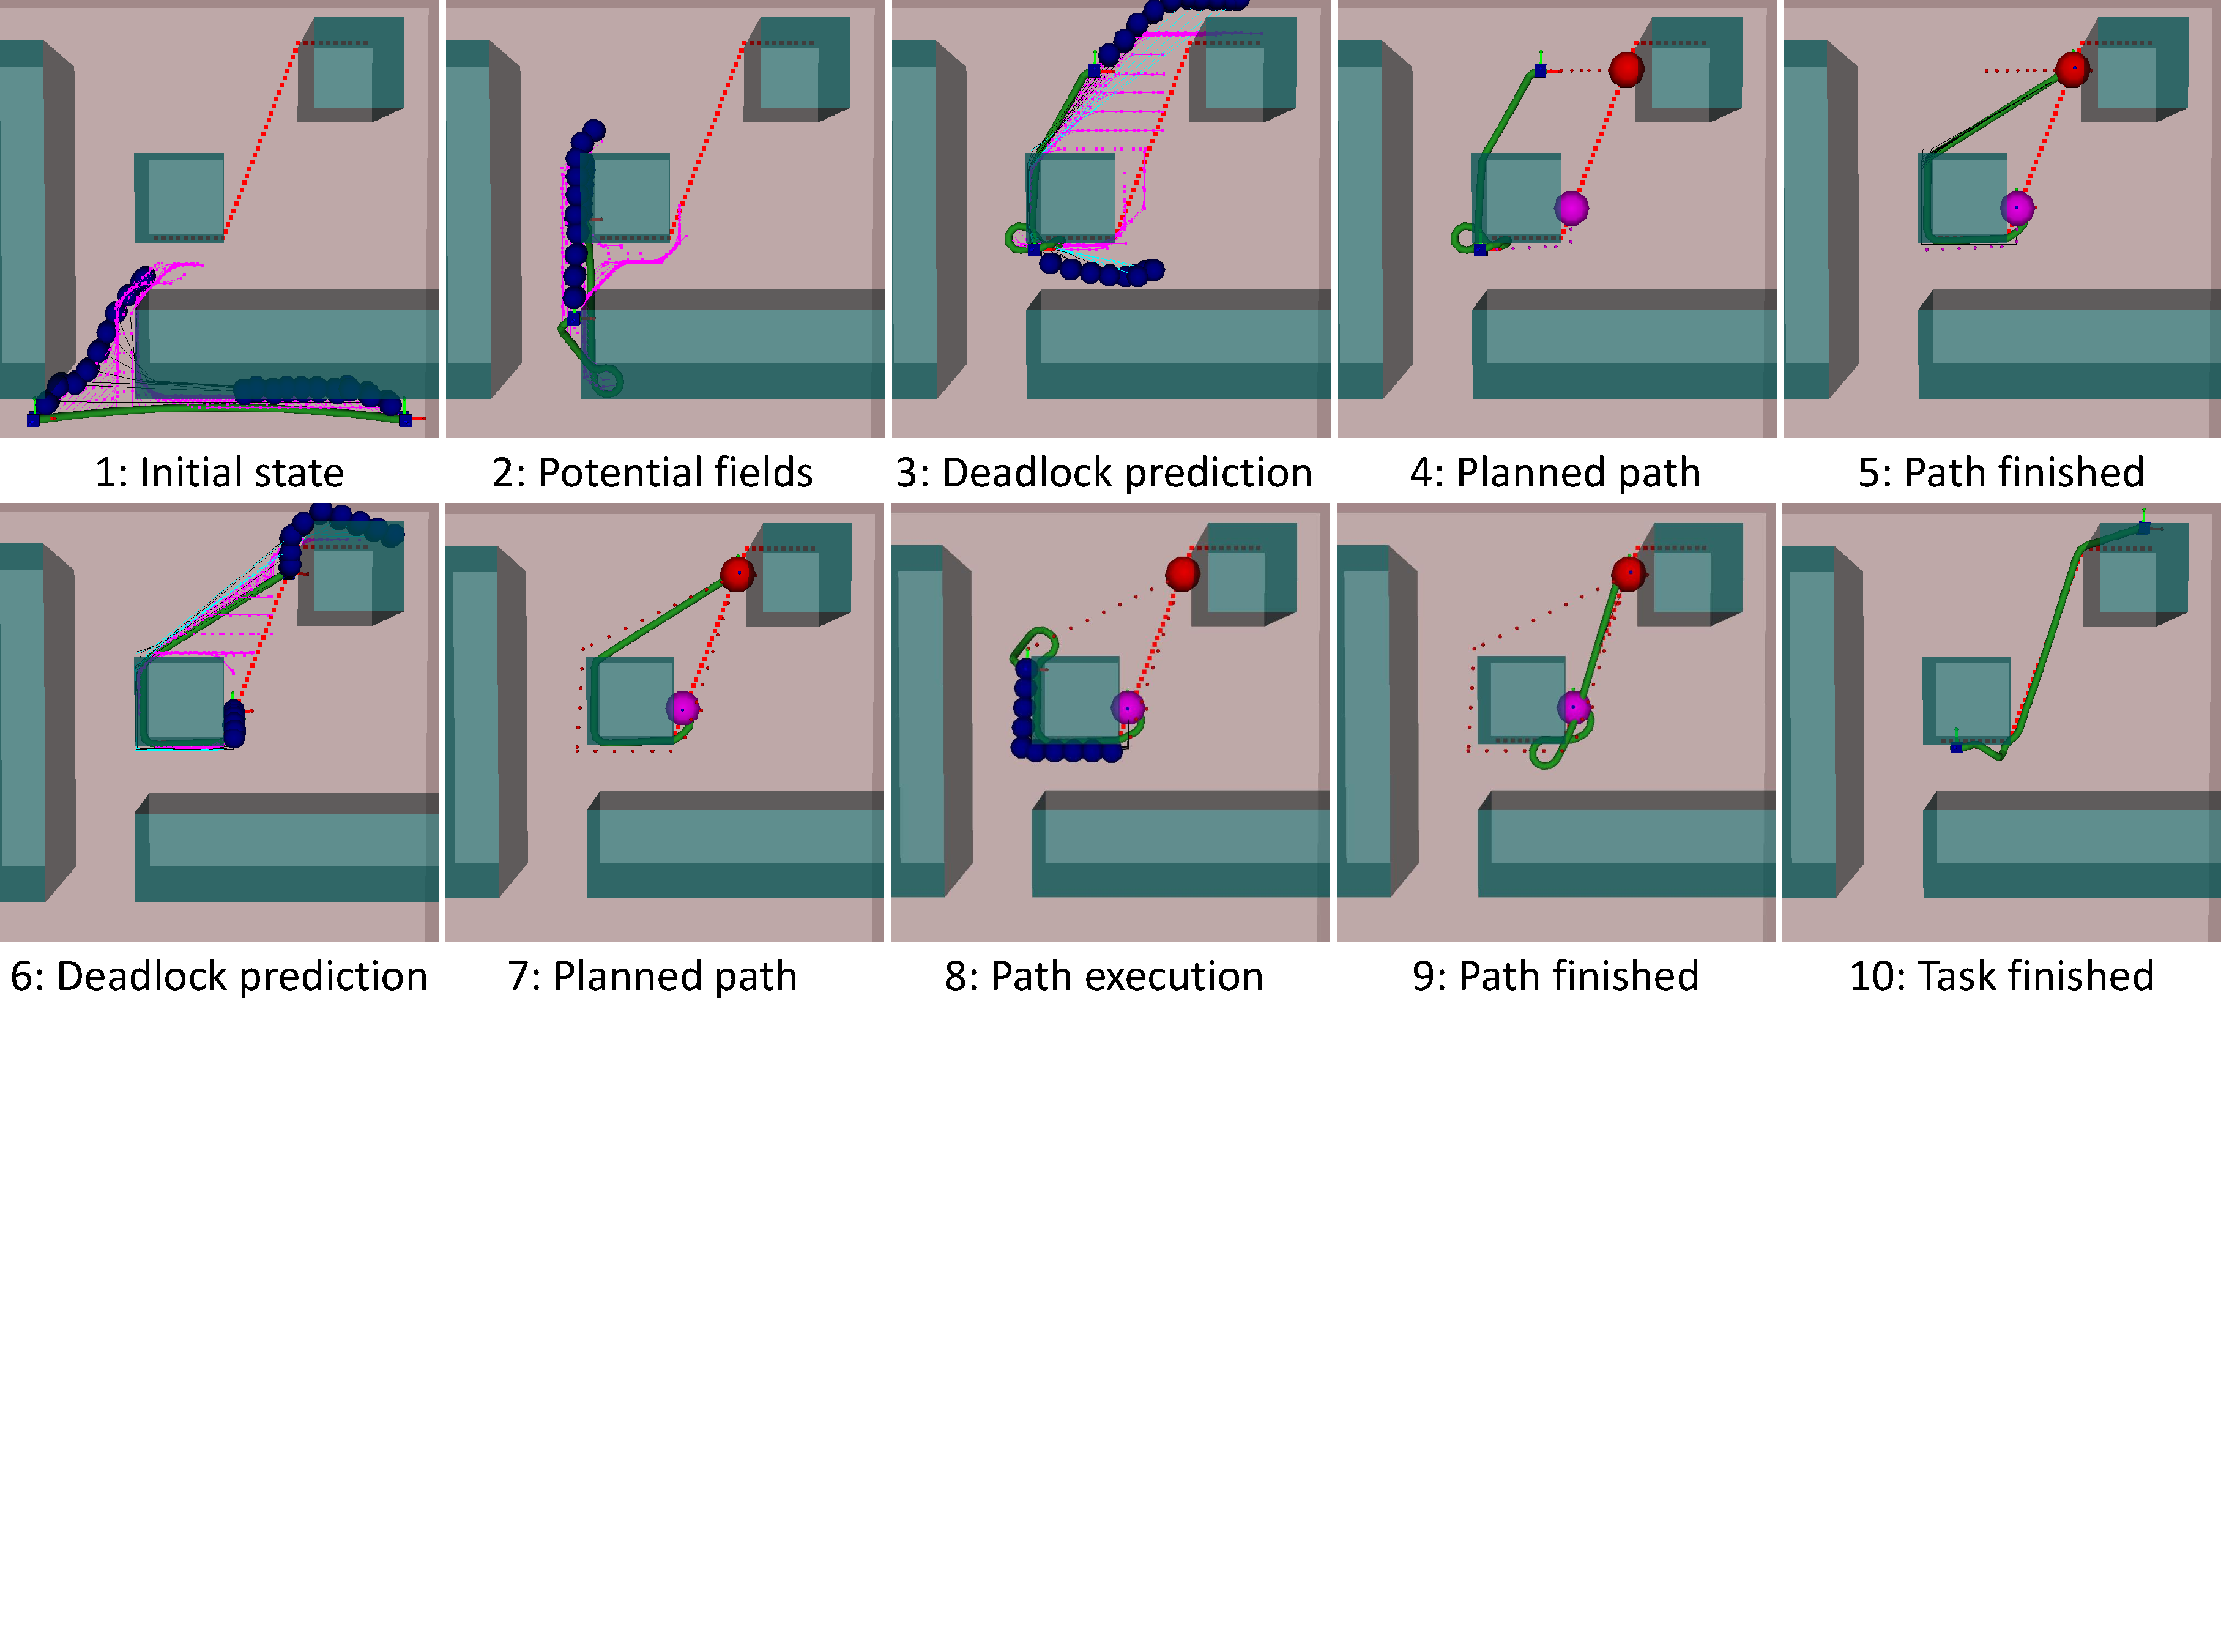
\includegraphics[width=\textwidth]{CombinedImages_RepeatedPlanning}
    \vspace{-2in}
    \caption{Sequence of snapshots for the fourth experiment. We use the same colors as the previous experiment (Figure~\ref{fig:rope_maze}), but in this example the local controller gets stuck twice, in panels 3 and 6. In panel 7 the global planner finds a new neighbourhood that is distinct from previously-tried neighbourhoods.}
    \label{fig:repeated_planning}
\end{figure}

\FloatBarrier

\begin{table}[h]
\centering
\caption{Planning statistics for the first plan for each example task in simulation, averaged across 100 trials. Standard deviation is shown in brackets.}
\label{tab:planning_statistics}
\begin{tabular}{lccccc}
\hline\noalign{\smallskip}
    & Samples & States & \makecell{NN\\Time\\(s)} & \makecell{Validity\\Checking\\Time (s)} & \makecell{Total\\Time\\(s)} \\
\noalign{\smallskip}\hline\noalign{\smallskip}
Single Pillar                    & \makecell{ 158 \\ {[121]}} & \makecell{1182 \\ {[804]}} & \makecell{$\sim$0.0 \\{[$\sim$0.0]}} & \makecell{0.6 \\{[0.5]}} & \makecell{0.6 \\{[0.5]}}\\
\noalign{\smallskip}
Double Slit                      & \makecell{ 478 \\ {[353]}} & \makecell{2124 \\{[1428]}} & \makecell{$\sim$0.0 \\{[$\sim$0.0]}} & \makecell{0.7 \\{[0.8]}} & \makecell{0.7 \\{[0.8]}}\\
\noalign{\smallskip}
Rope Maze                        & \makecell{4796 \\{[1613]}} & \makecell{9926 \\{[3760]}} & \makecell{      0.1 \\{[$\sim$0.0]}} & \makecell{4.0 \\{[1.7]}} & \makecell{4.2 \\{[1.8]}}\\
\noalign{\smallskip}
\makecell[l]{Repeated\\Planning} & \makecell{54   \\  {[46]}} & \makecell{153  \\ {[147]}} & \makecell{$\sim$0.0 \\{[$\sim$0.0]}} & \makecell{0.1 \\{[0.1]}} & \makecell{0.1 \\{[0.1]}}\\
\noalign{\smallskip}\hline
\end{tabular}
\end{table}

\begin{table}[h]
\centering
\caption{Smoothing statistics for the first plan for each example task in simulation, averaged across 100 trials. Standard deviation is shown in brackets.}
\label{tab:smoothing_statistics}
\begin{tabular}{lcccc}
\hline\noalign{\smallskip}
    & Iterations & \makecell{Validity\\Checking\\Time (s)} & \makecell{Visibility\\Deformation\\Time (s)}& \makecell{Total\\Time\\(s)}\\
\noalign{\smallskip}\hline\noalign{\smallskip}
Single Pillar                    &  500 & \makecell{0.8 \\{[1.2]}} & \makecell{       1.6 \\{[0.2]}}       & \makecell{2.4 \\{[1.2]}}\\
\noalign{\smallskip}
Double Slit                      &  500 & \makecell{2.5 \\{[2.6]}} & \makecell{$\sim$ 0.0 \\{[$\sim$0.0]}} & \makecell{2.5 \\{[2.6]}}\\
\noalign{\smallskip}
Rope Maze                        & 1500 & \makecell{6.4 \\{[3.9]}} & \makecell{$\sim$ 0.0 \\{[$\sim$0.0]}} & \makecell{6.5 \\{[3.9]}}\\
\noalign{\smallskip}
\makecell[l]{Repeated\\Planning} &  500 & \makecell{1.4 \\{[0.9]}} & \makecell{$\sim$ 0.0 \\{[$\sim$0.0]}} & \makecell{1.4 \\{[0.9]}}\\
\noalign{\smallskip}\hline
\end{tabular}
\end{table}

\FloatBarrier

\subsection{Computation Time}

To verify the practicality of our deadlock prediction algorithm and VEB approximation, we gathered data comparing computation time for these components to the local controller by itself, and to using the Bullet simulator. Table~\ref{tab:control_statistics} shows the average times per iteration for the local controller and deadlock prediction algorithms, averaged across all trials of all experiments. As expected, adding in the deadlock prediction step does increase computation time, but the overall control loop is still fast enough for practical use.

\begin{table}[h]
\centering
\caption{Local controller and deadlock prediction avg. computation time per iteration for each type of deformable object, averaged across all trials.}
\label{tab:control_statistics}
\begin{tabular}{lccc}
\noalign{\smallskip}\hline\noalign{\smallskip}
& 
\parbox{1.3in}{\centering Calculate\\Correspondences()\\Time (s)} &
\parbox{0.8in}{\centering Predict\\Deadlock() Time (s)} &
\parbox{0.8in}{\centering Local\\Controller Time (s)} \\
\noalign{\smallskip}\hline\noalign{\smallskip}
Cloth   & 0.0114 & 0.0077 & 0.0126 \\
Rope    & 0      & 0.0119 & 0.0023 \\
\noalign{\smallskip}\hline
\end{tabular}
\end{table}

\begin{table}[h]
\centering
\caption{Average computation time to compute the effect of a gripper motion.}
\label{tab:prediction_statistics}
\begin{tabular}{lcc}
\noalign{\smallskip}\hline\noalign{\smallskip}
& 
\parbox{1.7in}{\centering Bullet Simulation\\Time (ms)} &
\parbox{2in}{\centering VEB Propagation\\Time (ms)} \\
\noalign{\smallskip}\hline\noalign{\smallskip}
Cloth   & 36.12 & 0.19 \\
Rope    &  3.19 & 0.58 \\
\noalign{\smallskip}\hline
\end{tabular}
\end{table}

Table~\ref{tab:prediction_statistics} shows a comparison between the average time needed to compute the VEB propagation for a gripper motion and the time needed to reliably simulate a gripper motion with the Bullet simulator. Note that the amount of time required for the simulator to converge to a stable estimate depends on many conditions, including what object is being simulated. Through experimentation we determined that 4 simulation steps were adequate for rope and 10 for cloth. Comparing the time needed to do this simulation to the time needed to forward propagate a VEB, we see that our approximation is indeed faster by an order of magnitude for rope, and by two orders of magnitude for cloth. This result reinforces the importance of using a simplified model, such as the VEB, within the planner---this model, while not as accurate as a simulation, allows us to evaluate motions much faster.




%%%%%%%%%%%%%%%%%%%%%%%%%%%%%%%%%%%%%%%%%%%%%%%%%%%%%%%%%%%%%%%%%%%%%%%%%%%%%%%

\section{Physical Robot Experiment and Results}
\label{sec:live_robot}

In order to show that our method is practical for a physical robotic system, not only free floating end-effectors, we set up a task similar to the single pillar task (Section~\ref{sec:single_pillar}) with a dual-arm robot. It also shows that while our methods strong assumptions about the ability to perceive the deformable object in Section~\ref{sec:main_problem_statement} (in particular no occlusions and no sensor noise), our framework is still able to perform meaningful tasks when those assumptions are violated. In this task the robot must align a cloth placemat inside of the pink rectangle, going around an obstacle in the process (Figure~\ref{fig:cloth_placemat}).

\begin{figure}[h]
    \centering
    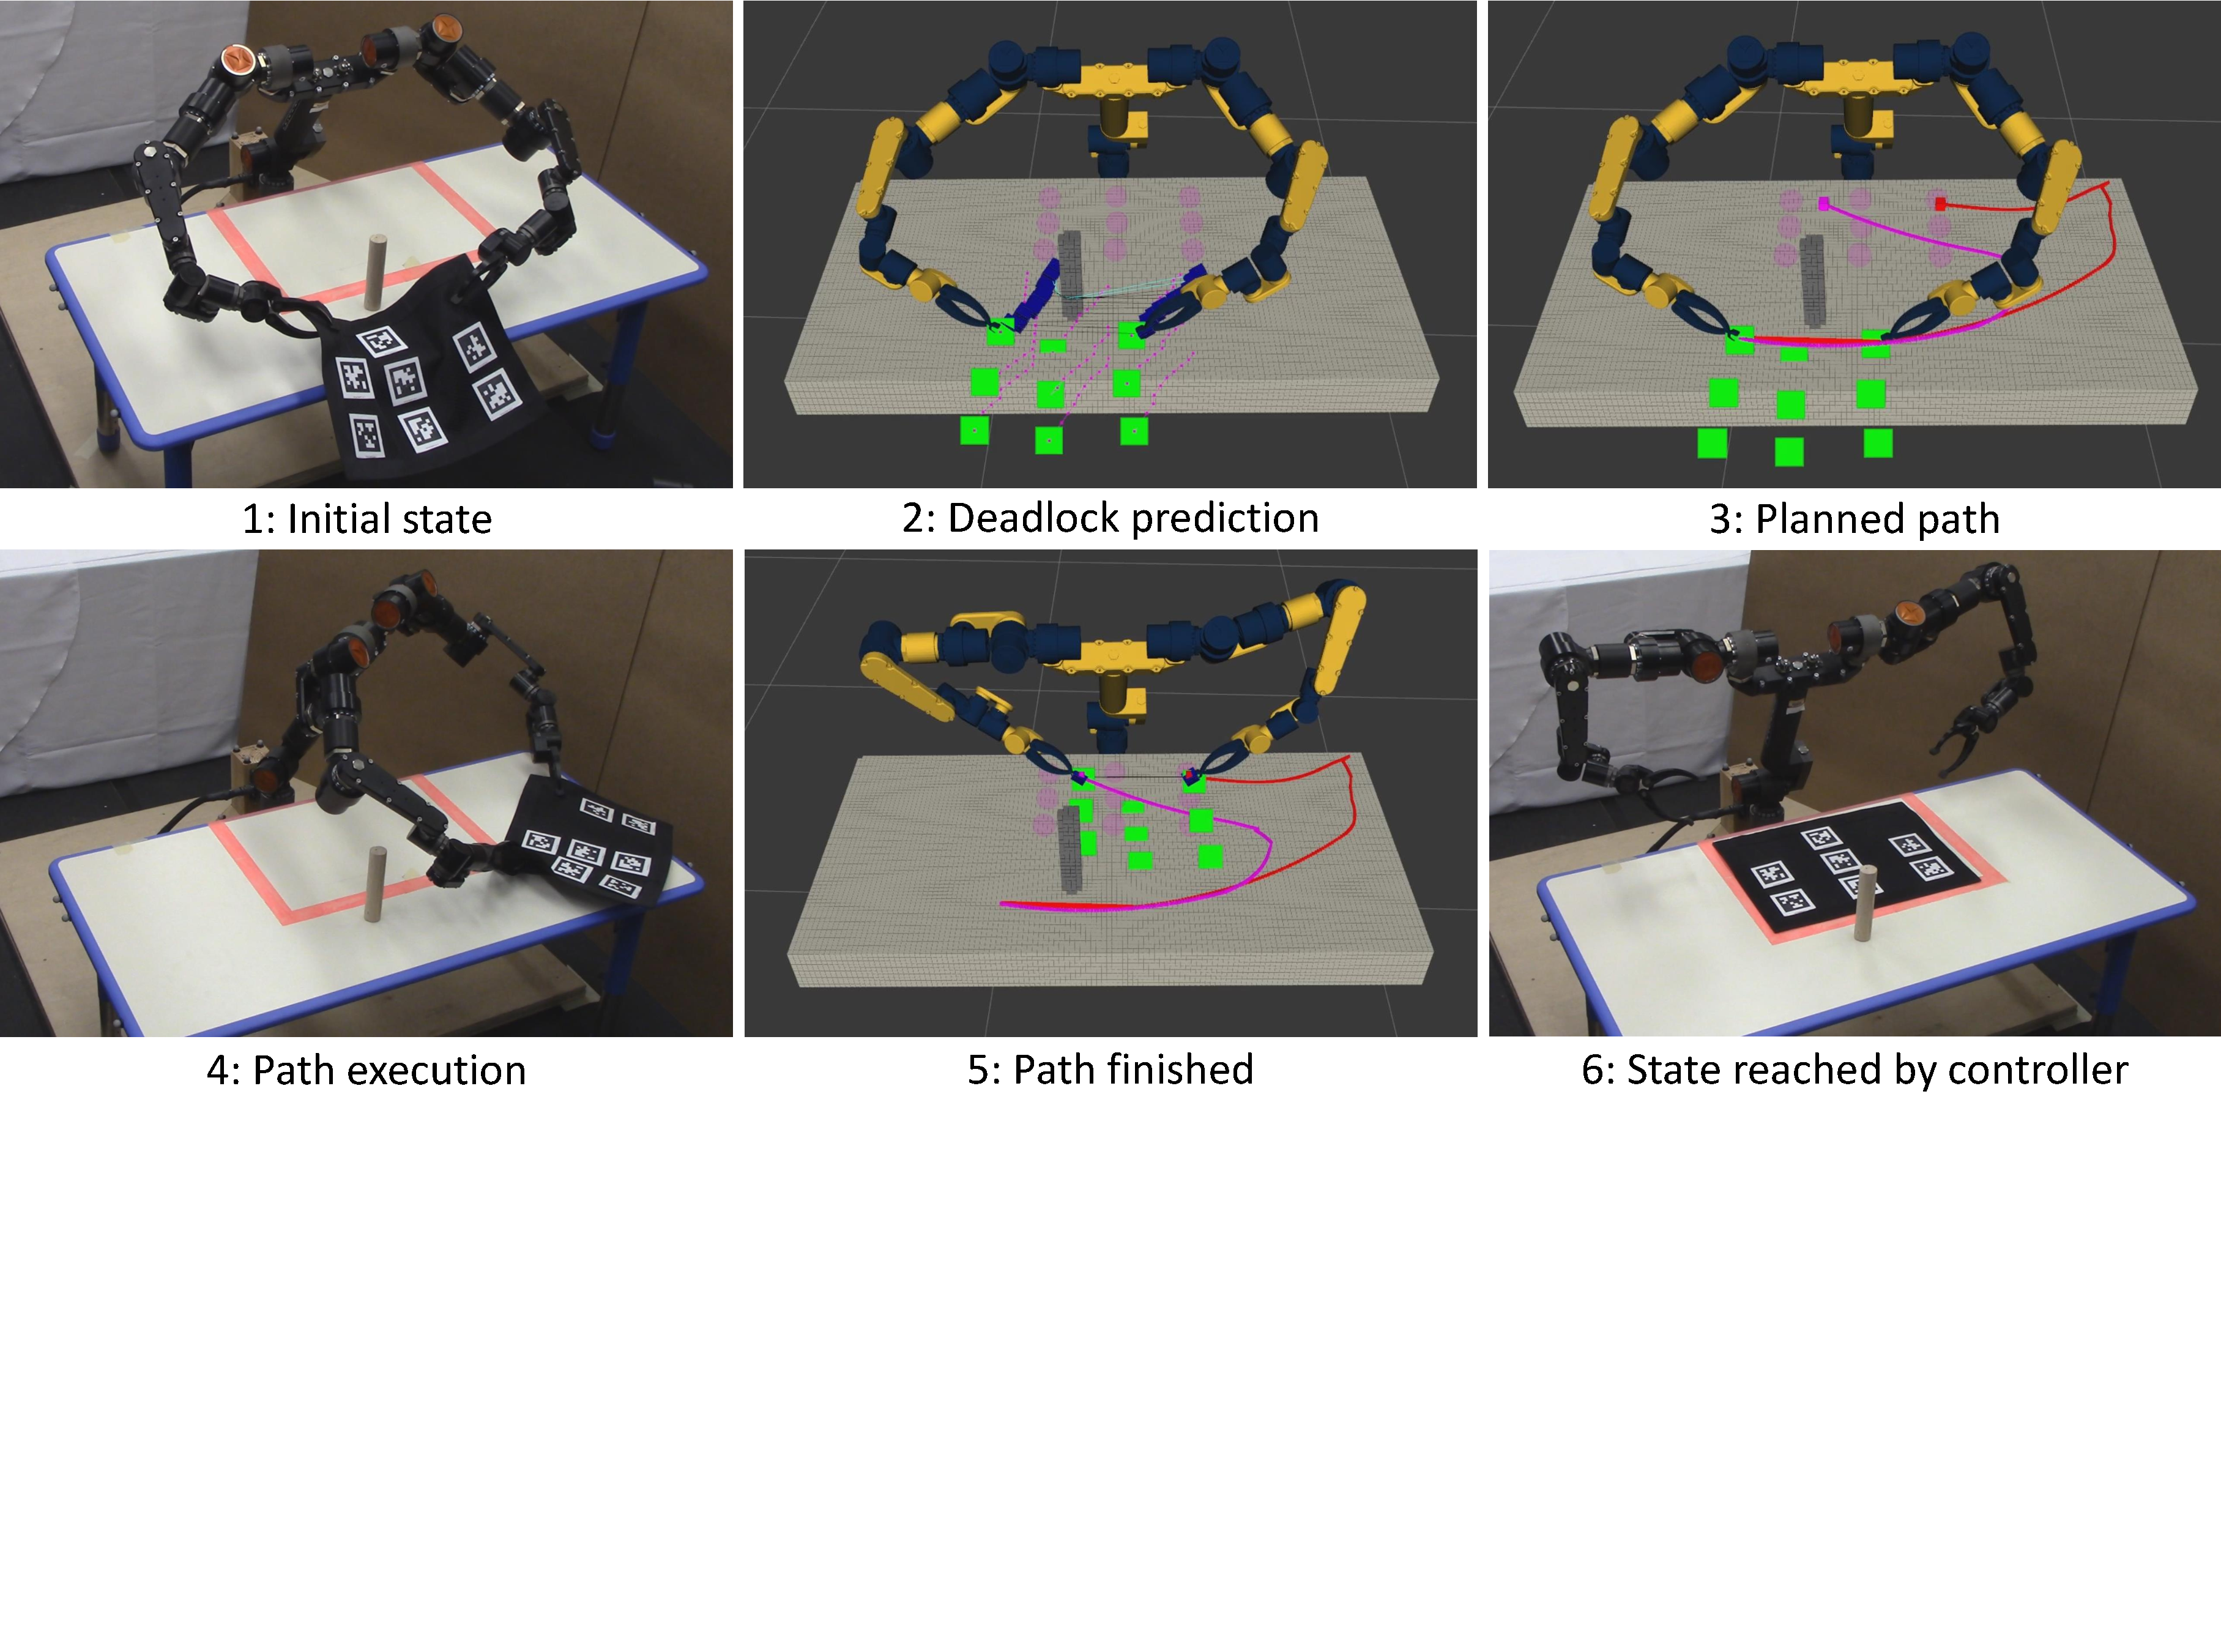
\includegraphics[width=\textwidth]{CombinedImages_LiveRobot}
    \vspace{-1.7in}
    \caption{Cloth placemat task. The placemat starts on the far side of an obstacle and must be aligned with the pink rectangle near the robot.}
    \label{fig:cloth_placemat}
\end{figure}

\subsection{Experiment Setup}

\subsubsection{Robotic Platform:}
Val is a stationary robotic platform with a 2-DOF torso, two 7-DOF arms, and a rotary pincer per arm. As in the simulated environments it is assumed that Val is already holding the cloth, leaving 16 DOF to be controlled and planned for ($\robotCspace = \reals^{16})$.


\subsubsection{Cloth Perception:}
\label{sec:cloth_perception}

The placemat is $0.33\text{m} \times 0.46\text{m}$ which we discretize into a $3 \times 3$ grid. As tracking of deformable objects is a difficult problem, and out of scope of this paper, we instead use fiducials to track the configuration of the cloth. Two of the points are tracked using the position of the grippers; the other 7 points are tracked with AprilTags~\cite{olson2011tags} and a Kinect V2 RGB-D sensor~\cite{iai_kinect2}.

In order to address occlusions and noisy data, we filter the raw observations using a set of objective terms, and a set of constraints (see Figure~\ref{fig:cloth_estimation}). Denote $z_i$ as the last observed position of point $i$, and denote $t_i$ as the last time point $i$ was observed. Then we add objective terms to pull the cloth estimate towards the observations, combined with constraints between each pair of points to ensure that the estimate is plausible:
\begin{equation}
\begin{aligned}
    \deformconfig(t) = &\argmin_{\{ p_i \}} 
            & & \sum_i e^{-K_T(t - t_i)} \| p_i - z_i \|^2 \\
            & \text{subject to}
            & & \| p_i - p_j \|^2 \leq K_L d_{ij}^2 \enspace \forall i, j \text{ s.t. } i \neq j \enspace .
\end{aligned}
\label{eqn:cloth_estimation}
\end{equation}
$K_T$ and $K_L$ are task defined scale factors which we set to $1.5$ and $1.0001$ respectively for this task.

\begin{figure}[h]
    \centering
    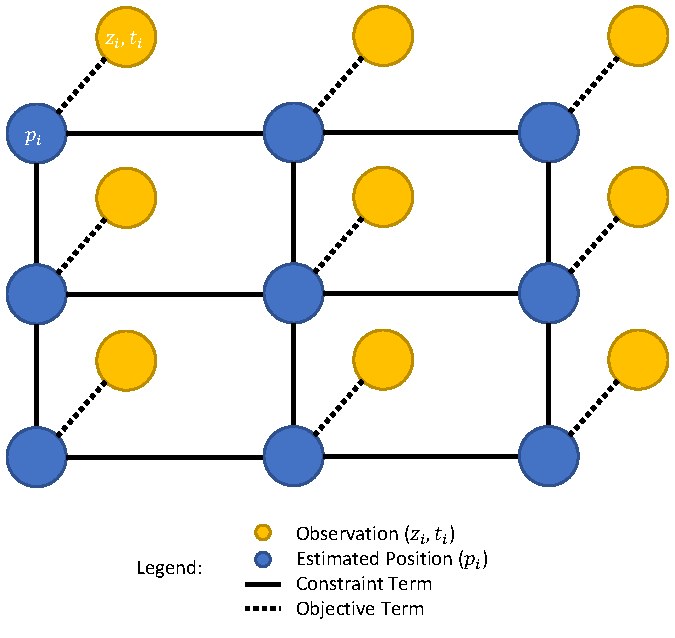
\includegraphics[width=0.6\columnwidth]{ClothEstimation}
    \caption{Constraint and objective graph for Eq.~\eqref{eqn:cloth_estimation}. Note that not all constraints are shown to avoid clutter; every estimated position has a constraint between itself and every other estimated position.}
    \label{fig:cloth_estimation}
\end{figure}

\subsection{Experiment Results}

We use the same deadlock, distance, and planner parameters as used in the simulation experiments, performing 500 smoothing iterations once a path is found. We constrain the rotation of the end-effectors to stay within 1.6 radians of their starting orientation during the planning process as well as constrain the grippers to stay close to the table. This forces the planner to move the placemat around the obstacle rather than over the obstacle. Last, we also introduce planning restarts \cite{Wedge2008} into the planning process in order to address the greater complexity added by using a 16-DOF robot and the relatively strict workspace constraints; the restart timeout we set is 60 seconds.

Tables~\ref{tab:live_robot_stats_planning} and \ref{tab:live_robot_stats_smoothing} show the planning and smoothing statistics across 100 planning trials with identical starting configurations, but different random seeds. On average planning and smoothing takes less than 60 seconds, with forward kinematics and collision checking dominating the planning time. The restart timeout was unused in 68 out of 100 trials, with the other 32 trials requiring a total of 50 restarts between them. Figure~\ref{fig:placemat_planning_time} shows that the planning time follows a ``heavy tail'' distribution typical of sampling-based planners.

\begin{table*}[h]
\centering
\caption{Planning statistics for the cloth placemat example, averaged across 100 trials. Standard deviation is shown in brackets.}
\label{tab:live_robot_stats_planning}
\begin{tabular}{cccccc}
\noalign{\smallskip}\hline\noalign{\smallskip}
Samples & 
States &
\makecell{NN\\Time\\(s)} & 
\makecell{Validity\\Checking\\Time (s)} & 
\makecell{Random\\Restarts} &
\makecell{Total\\Time\\(s)} \\
\noalign{\smallskip}\hline\noalign{\smallskip}
\makecell{83041\\{[83677]}} &
\makecell{8438\\{[6182]}} &
\makecell{4.5\\{[4.9]}} &
\makecell{44.1\\{[44.5]}} &
\makecell{0.5\\{[0.9]}} &
\makecell{50.0\\{[50.9]}} \\
\noalign{\smallskip}\hline
\end{tabular}
\end{table*}

\begin{table}[h]
\centering
\caption{Smoothing statistics for the cloth placemat example, averaged across 100 trials. Standard deviation is shown in brackets.}
\label{tab:live_robot_stats_smoothing}
\begin{tabular}{cccc}
\noalign{\smallskip}\hline\noalign{\smallskip}
Iterations & 
\makecell{Validity\\Checking\\Time (s)} &
\makecell{Visibility\\Deformation\\Time (s)} &
\makecell{Total\\Time\\(s)} \\
\noalign{\smallskip}\hline\noalign{\smallskip}
500 &
\makecell{3.6\\{[1.1]}} &
\makecell{0.1\\{[$\sim$0.0]}} &
\makecell{3.6\\{[1.1]}} \\
\noalign{\smallskip}\hline
\end{tabular}
\end{table}

\begin{figure}[h]
    \centering
    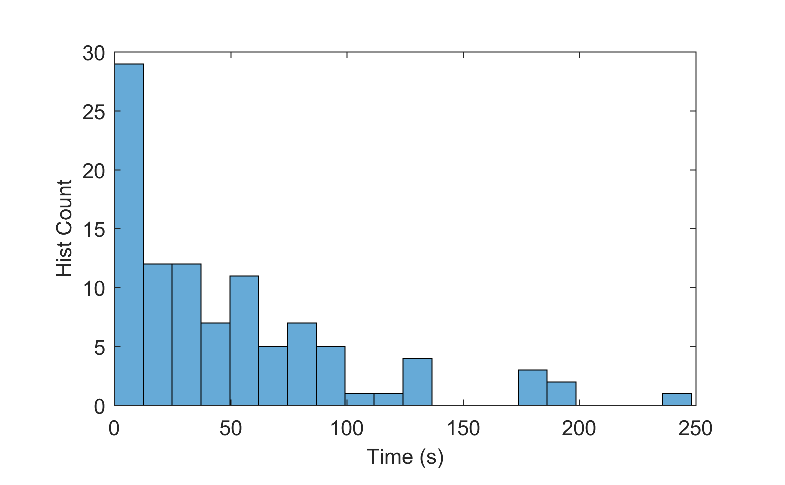
\includegraphics[width=0.7\columnwidth]{placemat_planning_total_time}
    \caption{Histogram of planning times across 100 trials for the cloth placemat experiment.}
    \label{fig:placemat_planning_time}
\end{figure}

Our overall framework is able to complete this task as shown in Figure~\ref{fig:cloth_placemat}. As in the simulated version of this task, we are able to predict deadlock before the robot gets stuck, plan and execute a path to a new neighbourhood, and then use the local controller to finish the task.
